\chapter{Công cụ và môi trường thực hiện}
Trong trương này em sẽ trình bày những công cụ và môi trường cần thiết trong quá trình huấn luyện mô hình \acrshort*{ocr}. Dưới đây là các bước trình bày chi tiết:
\begin{enumerate}
    \item \textbf{Phầm mềm và công cụ hỗ trợ:} Trình bày các phầm mềm và công cụ cho quá trình chuẩn bị dữ liệu, huấn luyện và xây dựng mô hình.
    \item \textbf{Tạo môi trường và cài công cụ cần thiết}: Trình bày các bước cài đặt môi trường cho đề tài và thiết lập một số môi trường cần thiết để chạy.

\end{enumerate}

Các công cụ và môi trường là nền tảng quan trọng cho việc thực hiện nghiên cứu, giúp định hình cách tiến hành các bước quan trọng trong đề tài ``Nghiên cứu ứng dụng công nghệ OCR nhận dạng hóa đơn''.

\section{Phầm mềm và công cụ hỗ trợ}
\subsection{Google Colab}
Google Colab (viết tắt của Google Colaboratory) là một dịch vụ miễn phí của Google cho phép thực hiện và chia sẻ các tệp notebook Jupyter, cũng như code Python. Nó là một môi trường trực tuyến, cho phép người dùng viết và chạy code Python một cách trực tiếp trên trình duyệt web mà không cần cài đặt bất kỳ môi trường phát triển nào trên máy tính.

Colab cung cấp sử dụng miễn phí cho CPU, GPU và RAM để người dùng có thể thực hiện các nhiệm vụ tính toán phức tạp mà không cần phải mua hoặc cấu hình phần cứng riêng. Colab còn được tích hợp sẵn với nhiều thư viện phổ biến cho khoa học dữ liệu, học máy và xử lý ảnh, giúp dễ dàng tiến hành các tác vụ phức tạp. Có thể tạo notebook Jupyter, trong đó bạn có thể viết code Python từng cell và thực thi chúng một cách tương tác. Điều này rất hữu ích cho việc thử nghiệm, phân tích dữ liệu và xây dựng mô hình máy học.

Colab có thể chia sẻ notebook của mình với người khác thông qua liên kết. Người khác có thể xem và chỉnh sửa notebook hoặc thậm chí làm việc chung với nhau trên cùng một notebook. Có thể lưu notebook và dữ liệu của mình trực tiếp vào Google Drive để truy cập dễ dàng và chia sẻ với các thiết bị khác.

Google Colab thường được sử dụng trong việc học, nghiên cứu và phát triển các dự án liên quan đến khoa học dữ liệu, học máy và trí tuệ nhân tạo mà không cần đầu tư nhiều vào cấu hình phần cứng.

\subsection{Vast.ai}
Vast.ai là một nền tảng tính toán phi tập trung cho phép bất cứ ai cho thuê công suất tính toán dư thừa của mình để kiếm tiền. Nó kết nối những người cần công suất tính toán bổ sung cho các tác vụ như học máy với những người có GPU hoặc CPU nhàn rỗi trên máy tính của họ. Một số tính năng chính của Vast.ai:

\begin{itemize}
    \item Mạng phi tập trung: Vast.ai chạy trên mạng ngang hàng phi tập trung thay vì máy chủ tập trung. Điều này làm cho nó bền vững và minh bạch hơn.
    \item Cho thuê công suất tính toán dư thừa: Mọi người có thể cài đặt ứng dụng khách Vast.ai trên máy tính của họ để cho thuê bất kỳ chu kỳ GPU hoặc CPU không sử dụng nào và được trả bằng tiền điện tử. Điều này cho phép mọi người kiếm tiền từ các tài nguyên tính toán dư thừa.
    \item Thuê công suất tính toán: Các nhà nghiên cứu, nhà phát triển và những người khác cần công suất tính toán bổ sung cho các ứng dụng như huấn luyện học máy có thể thuê GPU và CPU theo yêu cầu thông qua sàn giao dịch vast.ai. Giá được định giá động dựa trên cung và cầu.
    \item Mã nguồn mở: Vast.ai là một dự án nguồn mở được xây dựng trên các công nghệ phi tập trung hiện có. Điều này cho phép tính minh bạch và đóng góp của cộng đồng vào nền tảng.
\end{itemize}
Vast.ai tạo ra mô hình kinh tế chia sẻ cho công suất tính toán, kết nối những người có nguồn lực dư thừa với những người cần chúng theo cách ngang hàng phi tập trung. Nó cung cấp một cách dễ dàng để bất cứ ai có thể kiếm tiền từ công suất tính toán không sử dụng.

\subsection{CUDA Toolkit}
CUDA Toolkit (Compute Unified Device Architecture Toolkit) là một bộ công cụ và thư viện phát triển bởi NVIDIA dành cho việc phát triển ứng dụng và tính toán sử dụng các GPU của NVIDIA. CUDA là một mô hình lập trình và nền tảng tích hợp vào GPU để thực hiện tính toán đồng thời và xử lý dữ liệu song song. Điều này cho phép các ứng dụng thực hiện tính toán nhanh hơn trên GPU so với việc sử dụng CPU truyền thống.

CUDA Toolkit bao gồm các thành phần quan trọng sau đây:
\begin{enumerate}
    \item \textbf{CUDA Runtime}: CUDA Runtime là một tập hợp các thư viện và API cho phép ứng dụng tương tác với GPU và thực hiện các phép tính trên GPU. Nó cho phép bạn chạy các chương trình CUDA trên GPU của NVIDIA.
    \item \textbf{CUDA Compiler}: CUDA Toolkit đi kèm với trình biên dịch nvcc để biên dịch mã CUDA C/C++ thành mã máy GPU thực thi được.
    \item \textbf{CUDA Libraries}: CUDA Toolkit cung cấp một loạt thư viện cho các loại tính toán khác nhau, bao gồm thư viện đại số tuyến tính, thư viện xử lý ảnh, thư viện tính toán máy học (cuDNN, cuBLAS), và nhiều thư viện khác.
    \item \textbf{CUDA SDK}: CUDA SDK cung cấp các ví dụ và tài liệu hướng dẫn để bạn có thể bắt đầu phát triển ứng dụng sử dụng CUDA.
    \item \textbf{NVIDIA GPU Driver}: CUDA Toolkit yêu cầu cài đặt đúng phiên bản driver cho GPU của bạn để hoạt động.
\end{enumerate}

CUDA Toolkit thường được sử dụng trong lĩnh vực deep learning, scientific computing, và các ứng dụng đòi hỏi tính toán song song và xử lý số lớn. Nó cho phép các nhà phát triển tận dụng sức mạnh của GPU để gia tăng hiệu suất tính toán và tốc độ xử lý dữ liệu cho các ứng dụng của họ.

\subsection{cuDNN}
Đây là một thư viện phần mềm do NVIDIA phát triển, được tối ưu hóa cho việc thực hiện các phép tính liên quan đến mạng nơ-ron trên GPU. Tên gọi "cuDNN" viết tắt của "CUDA Deep Neural Network library," cho thấy rằng nó được phát triển để hỗ trợ hiệu suất cao khi sử dụng GPU để huấn luyện và triển khai các mô hình mạng nơ-ron sâu (deep neural networks).

Thư viện cung cấp một loạt các chức năng và thư viện tối ưu hóa để thực hiện các phép tính phổ biến trong deep learning, bao gồm các phép tính như: Convolution, Pooling, Normalization, Activation, Recurrent, \ldots

cuDNN được tích hợp vào nhiều framework deep learning phổ biến như TensorFlow và PyTorch, giúp cải thiện hiệu suất huấn luyện và triển khai mô hình trên GPU. Nó đóng vai trò quan trọng trong việc tăng tốc quá trình huấn luyện và triển khai mô hình deep learning trên nền tảng GPU của NVIDIA.
\subsection{PaddleOCR}
PaddleOCR là một dự án mã nguồn mở do PaddlePaddle phát triển, nhằm cung cấp một giải pháp toàn diện cho các nhiệm vụ liên quan đến xử lý ảnh và văn bản, bao gồm cả nhận dạng ký tự, nhận dạng văn bản và các tác vụ liên quan đến OCR. Dự án này được xây dựng trên cơ sở của các mô hình học sâu và sử dụng các thuật toán tiên tiến để giải quyết các thách thức trong việc xử lý ảnh và văn bản.

PaddleOCR hỗ trợ nhiều tác vụ liên quan đến OCR như nhận dạng ký tự, nhận dạng văn bản và phân loại chữ viết tay. Có thể được đào tạo và sử dụng cho nhiều ngôn ngữ khác nhau, giúp phát triển ứng dụng OCR toàn cầu. Người dùng có thể tùy chỉnh và đào tạo lại các mô hình của PaddleOCR cho phù hợp với nhu cầu cụ thể của dự án.

PaddleOCR có thể hoạt động trên nhiều nền tảng khác nhau, bao gồm máy tính cá nhân, máy chủ và các môi trường đám mây. Dự án cung cấp một loạt các mô hình học sâu đã được đào tạo trước để giúp giải quyết các vấn đề liên quan đến xử lý ảnh và văn bản.

Dự án được tối ưu hóa để đạt hiệu suất cao và đáp ứng yêu cầu xử lý ảnh và văn bản trong thời gian thực.

Hơn nữa PaddleOCR là một dự án mã nguồn mở và có cộng đồng hỗ trợ sẵn sàng chia sẻ kiến thức, giải đáp thắc mắc và cùng nhau phát triển.

Tóm lại, cung cấp một giải pháp mạnh mẽ và linh hoạt cho các ứng dụng liên quan đến xử lý ảnh và văn bản, đặc biệt là trong lĩnh vực OCR. Điều này giúp đơn giản hóa và tối ưu hóa quá trình xây dựng hệ thống nhận dạng văn bản và thông tin từ các hình ảnh hóa đơn và tài liệu khác.

\subsection{PPOCRLabel}
PPOCRLabel là một công cụ hỗ trợ trong lĩnh vực xử lý ảnh và trí tuệ nhân tạo, được sử dụng để thực hiện công việc nhận dạng và đánh dấu vùng chứa văn bản trên ảnh. Đây là một dự án mã nguồn mở của PaddlePaddle, một thư viện học máy phát triển bởi Baidu. PaddleOCR nhằm mục tiêu xây dựng các mô hình nhận dạng ký tự trên ảnh với hiệu suất cao.

PPOCRLabel được tạo ra để hỗ trợ quá trình chuẩn bị dữ liệu cho việc huấn luyện mô hình nhận dạng văn bản. Việc chuẩn bị dữ liệu là một bước quan trọng trong quá trình phát triển mô hình học máy, và công cụ như PPOCRLabel giúp đơn giản hóa và tăng cường hiệu suất của quá trình này. Dưới đây là một số tính năng chính của PPOCRLabel \cite{ppocrlabel}:
\begin{enumerate}
    \item \textbf{Labeling vùng chứa văn bản:} PPOCRLabel cho phép người dùng vẽ các hộp giới hạn xung quanh các vùng chứa văn bản trên ảnh để đánh dấu vị trí của văn bản cần nhận dạng.
    \item \textbf{Labeling trích xuất từ khóa:} Người dùng có thể gán nhãn thông tin từ khóa để cho bài toán trích xuất thông tin chính.
    \item \textbf{Gắn nhãn văn bản:} Người dùng có thể gắn nhãn văn bản được nhận dạng trong các hộp giới hạn để cho biết nội dung của văn bản đó.
    \item \textbf{Chú thích cho bảng:} PPOCRLabel cung cấp cho người dùng chức năng chú thích bảng nhằm mục đích bóc tách cấu trúc của bảng dưới dạng hình ảnh và chuyển sang định dạng Excel
    \item \textbf{Chỉnh sửa và xem trước:} PPOCRLabel cung cấp giao diện để chỉnh sửa và xem trước dữ liệu đã được đánh dấu trên ảnh, đảm bảo rằng dữ liệu được chuẩn bị chính xác trước khi sử dụng để huấn luyện mô hình.
    \item \textbf{Xuất dữ liệu:} Sau khi hoàn thành việc đánh dấu và chuẩn bị dữ liệu, PPOCRLabel cho phép bạn xuất dữ liệu trong các định dạng phổ biến để sử dụng trong quá trình huấn luyện mô hình.
    \item \textbf{Tích hợp với PaddleOCR:} PPOCRLabel có thể liên kết với dự án PaddleOCR để tiện lợi trong việc sử dụng dữ liệu đã được chuẩn bị để huấn luyện các mô hình nhận dạng văn bản.
\end{enumerate}

PPOCRLabel là một công cụ cực kỳ hữu ích trong quá trình chuẩn bị dữ liệu cho việc huấn luyện mô hình liên quan đến OCR, giúp tăng cường hiệu suất và chính xác của mô hình cuối cùng.

\subsection{Pytorch}
PyTorch là một thư viện mã nguồn mở được phát triển bởi Facebook's AI Research lab dùng cho việc xây dựng và huấn luyện các mạng nơ-ron. Nó được thiết kế đặc biệt để hỗ trợ tính toán trên mạng nơ-ron và dự án thực tế với sự linh hoạt và hiệu suất cao. PyTorch là một trong những thư viện phổ biến nhất cho deep learning và machine learning trong cộng đồng nghiên cứu và phát triển AI.

Một số điểm mạnh của PyTorch bao gồm:
\begin{enumerate}
    \item Tính năng tạo đồ thị động: PyTorch sử dụng một cơ chế đồ thị tính toán động, cho phép bạn xây dựng và điều chỉnh mô hình một cách linh hoạt trong quá trình chạy. Điều này rất hữu ích khi bạn cần xây dựng các mô hình phức tạp hoặc thực hiện các thay đổi động.
    \item Hỗ trợ GPU: PyTorch có tích hợp sẵn hỗ trợ tính toán trên GPU, giúp gia tăng tốc độ huấn luyện mô hình đáng kể.
    \item Cộng đồng phát triển mạnh mẽ: PyTorch có một cộng đồng người dùng và phát triển đông đảo, nên bạn có thể tìm thấy nhiều tài liệu học tập và hỗ trợ từ cộng đồng.
    \item Sử dụng dễ dàng: PyTorch có một cú pháp Python thân thiện và dễ đọc, giúp người dùng dễ dàng hiểu và sử dụng.
\end{enumerate}
PyTorch cung cấp các thành phần cơ bản để xây dựng và huấn luyện mạng nơ-ron, bao gồm tensor, autograd (tự động tính đạo hàm), và một loạt các lớp và hàm tiện ích để xây dựng mô hình. Nó đã trở thành một trong những công cụ quan trọng cho nghiên cứu và phát triển trong lĩnh vực deep learning.

\subsection{Gradio}
Gradio là một thư viện mã nguồn mở được sử dụng để xây dựng giao diện người dùng cho các mô hình học máy và học sâu một cách dễ dàng và nhanh chóng. Thư viện này giúp tạo ra các ứng dụng web hoặc desktop đơn giản để tương tác với các mô hình đã huấn luyện mà bạn đã xây dựng hoặc sử dụng.

Thư viện cung cấp một API Python dễ sử dụng để bạn có thể định nghĩa các giao diện người dùng tương tác cho các mô hình học máy và học sâu của mình. Với Gradio, ta có thể tạo các biểu đồ, hộp văn bản, nút bấm và các phần tử UI khác để tương tác với mô hình. Gradio cũng hỗ trợ việc hiển thị kết quả và dự đoán từ mô hình trực tiếp trong giao diện người dùng.

Gradio được thiết kế để đơn giản hóa việc tạo giao diện người dùng cho các mô hình học máy mà không cần kiến thức về phát triển web phức tạp. Tương thích với nhiều loại mô hình có thể sử dụng Gradio với các mô hình học máy, deep learning và thậm chí cả các mô hình không cần kết nối mạng. Hỗ trợ cả ứng dụng web và desktop, cho phép triển khai giao diện người dùng trên nhiều nền tảng.

Thư viện có khả năng tích hợp với các framework học máy và deep learning phổ biến như TensorFlow, PyTorch, và Scikit-Learn. Người dùng có thể tùy chỉnh giao diện người dùng của mình bằng cách thêm các phần tử UI và tuỳ chỉnh cách hiển thị kết quả.

Gradio giúp nhanh chóng tạo ra các ứng dụng tương tác cho các mô hình học máy của bạn mà không cần kiến thức chuyên sâu về phát triển giao diện người dùng. Điều này có thể rất hữu ích trong việc trình bày và thử nghiệm các mô hình với người dùng cuối.

\section{Cấu hình phần cứng}
Huấn luyện một mô hình học sâu đòi hỏi xử lý một lượng lớn dữ liệu và tính toán phức tạp. Cần phần cứng mạnh mẽ để xử lý nhanh chóng và hiệu quả. Phần cứng yếu sẽ làm chậm quá trình huấn luyện.Pphần cứng chất lượng cao cho phép huấn luyện nhanh hơn, với dữ liệu lớn hơn và mô hình phức tạp hơn. Do đó với từng tác vụ khác nhau em sẽ xử dụng một cấu hình khác nhau. Dưới đây là bảng so sánh phần cứng của từng tác vụ:

\begin{table}[h]
    \centering
    \begin{tabular}{| c | c | c | c |} 
     \hline
               & \textbf{Detection} & \textbf{KIE} & \textbf{Recognition} \\
     \hline\hline
     \textbf{Server}    & Colab & Colab & Vast.ai \\ 
     \textbf{OS}        & Ubuntu 22.04.2 & Ubuntu 22.04.2 & Ubuntu 22.04.2 \\
     \textbf{Python}    & 3.10 & 3.10 & 3.10 \\
     \textbf{CUDA}      & 12.0 & 12.0 & 11.7 \\
     \textbf{Framework} & PaddlePaddle & PaddlePaddle & Pytorch     \\
     \textbf{RAM}       & 13GB & 13GB & 64GB     \\
     \textbf{GPU}       & NVIDIA T4 & NVIDIA T4 & NVIDIA RTX 3060\\
     \hline
    \end{tabular}
    \caption{So sánh cấu hình phần cứng huấn luyện của từng tác vụ OCR}
    \label{table:hardward}
\end{table}

\section{Tạo môi trường và cài công cụ cần thiết}
\subsection{Cài đặt Miniconda:}
Miniconda là một công cụ quản lý môi trường và gói thư viện Python nhẹ và tối giản. Dưới đây là hướng dẫn cách tạo môi trường Miniconda trên hệ điều hành Ubuntu:

\textbf{Bước 1:} Tải Miniconda
\begin{lstlisting}[language=bash]
    wget https://repo.anaconda.com/miniconda/Miniconda3-latest-Linux-x86_64.sh
\end{lstlisting}

\textbf{Bước 2:} Cài đặt Miniconda
\begin{lstlisting}[language=bash]
    sh Miniconda3-latest-Linux-x86_64.sh    
\end{lstlisting}
Chấp nhận tất cả các điểu khoản
\begin{lstlisting}[language=bash]
    source ~/.bashrc
\end{lstlisting}

\textbf{Bước 3:} Tạo môi trường
\begin{lstlisting}[language=bash]
    conda create -n paddle_env python=3.8
\end{lstlisting}
Nhấn y để cài đặt

\textbf{Bước 4:} Kích hoạt môi trường
\begin{lstlisting}[language=bash]
    conda activate paddle_env
\end{lstlisting}
\begin{figure}[h]
    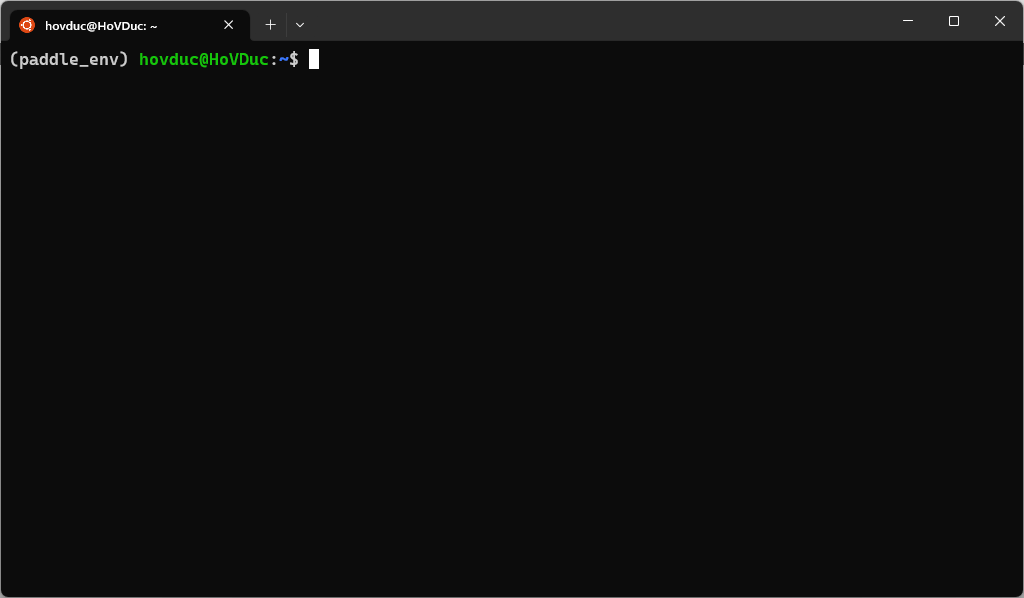
\includegraphics[scale=0.5]{images/terminal-conda-activate.png}    
    \centering
    \caption{Môi trường đã được kích hoạt}
\end{figure}

\subsection{Cài đặt CUDA Toolkit:}
\begin{lstlisting}[language=bash]
$ wget https://developer.download.nvidia.com/compute/cuda/repos/ubuntu2204/x86_64/cuda-ubuntu2204.pin
$ sudo mv cuda-ubuntu2204.pin /etc/apt/preferences.d/cuda-repository-pin-600
$ wget https://developer.download.nvidia.com/compute/cuda/11.7.0/local_installers/cuda-repo-ubuntu2204-11-7-local_11.7.0-515.43.04-1_amd64.deb
$ sudo dpkg -i cuda-repo-ubuntu2204-11-7-local_11.7.0-515.43.04-1_amd64.deb
$ sudo cp /var/cuda-repo-ubuntu2204-11-7-local/cuda-*-keyring.gpg /usr/share/keyrings/
$ sudo apt-get update
$ sudo apt-get -y install cuda
\end{lstlisting}

\subsection{Cài đặt cuDNN}
\textbf{Bước 1:} Tải xuống cuDNN
\begin{lstlisting}[language=bash]
wget https://developer.nvidia.com/downloads/compute/cudnn/secure/8.9.4/local_installers/11.x/cudnn-local-repo-ubuntu2204-8.9.4.25_1.0-1_amd64.deb
\end{lstlisting}

\textbf{Bước 2:} Cài đặt gói phần mềm
\begin{lstlisting}
sudo dpkg -i cudnn-local-repo-ubuntu2204-8.9.4.25_1.0-1_amd64.deb
\end{lstlisting}

\textbf{Bước 3:} Nhập khóa CUDA GPG
\begin{lstlisting}
sudo cp /var/cudnn-local-repo-*/cudnn-local-*-keyring.gpg /usr/share/keyrings/
\end{lstlisting}

\textbf{Bước 4:} Làm mới và cài đặt thư viện
\begin{lstlisting}
sudo apt-get update
sudo apt-get install libcudnn8=8.9.4.25_1.0-1+cuda11.7
sudo apt-get install libcudnn8-dev=8.9.4.25_1.0-1+cuda11.7
\end{lstlisting}


\subsection{Cài đặt PaddleOCR}
\textbf{Bước 1:} Cài đặt PaddlePaddle
\begin{lstlisting}[language=bash]
    python3 -m pip install paddlepaddle -i https://mirror.baidu.com/pypi/simple
\end{lstlisting}

\textbf{Bước 2:} Clone PaddleOCR và cài đặt
\begin{lstlisting}[language=bash]
    git clone https://github.com/PaddlePaddle/PaddleOCR.git
    pip install -r PaddleOCR/requirements.txt
\end{lstlisting}

\subsection{Cài đặt PPOCRLabel}
\begin{lstlisting}[language=bash]
    pip3 install PPOCRLabel
    pip3 install trash-cli
\end{lstlisting}

Trong chương này đã giới thiệu các công cụ và thư viện quan trọng trong đồ án. Phần tiếp theo em sẽ trình bày về dữ liệu và các bước huấn luyện mô hình OCR.